\documentclass[border={0pt -3pt 0pt 0pt}]{standalone}

\usepackage{hyperref}
\usepackage{tikz}

\usetikzlibrary{decorations.pathreplacing,
  arrows,
  calc,
  decorations.pathmorphing,
  decorations.pathreplacing,
  decorations.markings,
  positioning,
  shapes,
  3d
}

\tikzstyle{snakearrow} = [decorate, decoration={pre length=0.2cm,
  post length=0.2cm, snake, amplitude=.4mm,
  segment length=2mm},thick, ->]

\ifpdf
% Ensure reproducible output
\pdfinfoomitdate=1
\pdfsuppressptexinfo=-1
\pdftrailerid{}
\hypersetup{
  pdfcreator={},
  pdfproducer={}
}
\fi

\begin{document}
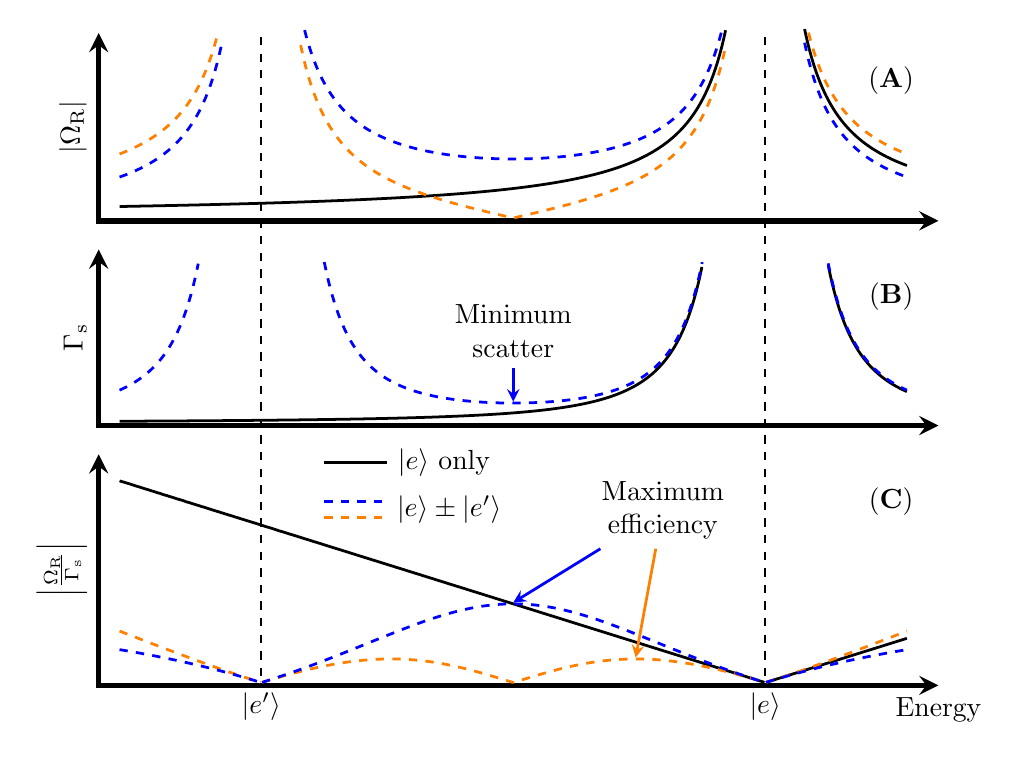
\begin{tikzpicture}[
  declare function={
    raman(\x,\a,\r) = \a / (\x - \r);
    raman1(\x) = raman(\x, 1.2, 3.2);
    raman2(\x,\s) = raman(\x, 1.2, 3.2) + \s * raman(\x, 1.2, -3.2);
    gamma(\x,\a,\r) = \a / (\x - \r)^2;
    gamma1(\x) = gamma(\x, 1.28, 3.2);
    gamma2(\x) = gamma(\x, 1.28, 3.2) + gamma(\x, 1.28, -3.2);
  }]

  \node[below] at (4.8, 8.25 - 0.3) {(\textbf{A})};
  \node[below] at (4.8, 5.5 - 0.3) {(\textbf{B})};
  \node[below] at (4.8, 2.9 - 0.3) {(\textbf{C})};

  \draw[dashed,line width=0.8] (3.2, 8.2) -- (3.2, 0) node[below] {$|e\rangle$};
  \draw[dashed,line width=0.8] (-3.2, 8.2) -- (-3.2, 0) node[below] {$|e'\rangle$};

  \draw[->,>=stealth,line width=2] (-5.3cm + 1pt, 5.9cm - 1pt) --
  node[rotate=90,above] {$\left|\Omega_{\mathrm{R}}\right|$} (-5.3cm + 1pt, 8.25);
  \draw[->,>=stealth,line width=2] (-5.3, 5.9cm - 1pt) -- (5.4, 5.9cm - 1pt);

  \draw[->,>=stealth,line width=2] (-5.3cm + 1pt, 3.3cm - 1pt) --
  node[rotate=90,above] {$\Gamma_{\mathrm{s}}$} (-5.3cm + 1pt, 5.5);
  \draw[->,>=stealth,line width=2] (-5.3, 3.3cm - 1pt) -- (5.4, 3.3cm - 1pt);

  \draw[->,>=stealth,line width=2] (-5.3cm + 1pt, 0cm - 1pt) --
  node[rotate=90,above] {$\left|\frac{\Omega_{\mathrm{R}}}{\Gamma_{\mathrm{s}}}\right|$}
  (-5.3cm + 1pt, 2.9);
  \draw[->,>=stealth,line width=2] (-5.3, 0cm - 1pt) -- (5.4, 0cm - 1pt)
  node[below] {Energy};

  \draw[line width=1] plot[samples=300,domain=-5:2.7,variable=\x] ({\x}, {abs(raman1(\x)) + 5.9});
  \draw[line width=1] plot[samples=700,domain=3.7:5,variable=\x] ({\x}, {abs(raman1(\x)) + 5.9});

  \draw[orange,dashed,line width=1]
  plot[samples=300,domain=-5:-3.75,variable=\x] ({\x}, {abs(raman2(\x, 1)) + 5.9});
  \draw[orange,dashed,line width=1]
  plot[samples=300,domain=-2.7:2.7,variable=\x] ({\x}, {abs(raman2(\x, 1)) + 5.9});
  \draw[orange,dashed,line width=1]
  plot[samples=300,domain=3.75:5,variable=\x] ({\x}, {abs(raman2(\x, 1)) + 5.9});

  \draw[blue,dashed,line width=1]
  plot[samples=300,domain=-5:-3.7,variable=\x] ({\x}, {abs(raman2(\x, -1)) + 5.9});
  \draw[blue,dashed,line width=1]
  plot[samples=300,domain=-2.65:2.65,variable=\x] ({\x}, {abs(raman2(\x, -1)) + 5.9});
  \draw[blue,dashed,line width=1]
  plot[samples=300,domain=3.7:5,variable=\x] ({\x}, {abs(raman2(\x, -1)) + 5.9});

  \draw[line width=1] plot[samples=300,domain=-5:2.4,variable=\x] ({\x}, {gamma1(\x) + 3.3});
  \draw[line width=1] plot[samples=700,domain=4.0:5,variable=\x] ({\x}, {gamma1(\x) + 3.3});

  \draw[blue,dashed,line width=1]
  plot[samples=300,domain=-5:-4.0,variable=\x] ({\x}, {gamma2(\x) + 3.3});
  \draw[blue,dashed,line width=1]
  plot[samples=300,domain=-2.4:2.4,variable=\x] ({\x}, {gamma2(\x) + 3.3});
  \draw[blue,dashed,line width=1]
  plot[samples=300,domain=4.0:5,variable=\x] ({\x}, {gamma2(\x) + 3.3});

  \draw[line width=1] plot[samples=300,domain=-5:3.19,variable=\x]
  ({\x}, {abs(raman1(\x) / gamma1(\x)) / 3});
  \draw[line width=1] plot[samples=700,domain=3.21:5,variable=\x]
  ({\x}, {abs(raman1(\x) / gamma1(\x)) / 3});

  \draw[orange,dashed,line width=1]
  plot[samples=300,domain=-5:-3.21,variable=\x] ({\x}, {abs(raman2(\x, 1) / gamma2(\x)) / 3});
  \draw[orange,dashed,line width=1]
  plot[samples=300,domain=-3.19:3.19,variable=\x] ({\x}, {abs(raman2(\x, 1) / gamma2(\x)) / 3});
  \draw[orange,dashed,line width=1]
  plot[samples=300,domain=3.21:5,variable=\x] ({\x}, {abs(raman2(\x, 1)) / gamma2(\x) / 3});

  \draw[blue,dashed,line width=1]
  plot[samples=300,domain=-5:-3.21,variable=\x] ({\x}, {abs(raman2(\x, -1) / gamma2(\x)) / 3});
  \draw[blue,dashed,line width=1]
  plot[samples=300,domain=-3.19:3.19,variable=\x] ({\x}, {abs(raman2(\x, -1) / gamma2(\x)) / 3});
  \draw[blue,dashed,line width=1]
  plot[samples=300,domain=3.21:5,variable=\x] ({\x}, {abs(raman2(\x, -1) / gamma2(\x)) / 3});

  \draw[line width=1] (-2.4, 2.8) -- (-1.6, 2.8) node[right] {$|e\rangle$ only};
  \draw[blue,dashed,line width=1] (-2.4, 2.3) -- (-1.6, 2.3);
  \draw[orange,dashed,line width=1] (-2.4, 2.1) -- (-1.6, 2.1);
  \node[right] at (-1.6, 2.2) {$|e\rangle\pm|e'\rangle$};

  \draw[<-,>=stealth,line width=1,blue] (0, 3.55cm + 0.5pt) -- (0, 4)
  node[black,above,align=center] {Minimum\\scatter};

  \node[black,above,align=center]
  at (1.9, 1.7) (BestRatioLabel) {Maximum\\efficiency};
  \draw[<-,>=stealth,line width=1,blue] (0, 3cm / 3 + 0.5pt) -- (BestRatioLabel);
  \draw[<-,>=stealth,line width=1,orange] (1.5547784696212665, 0.9008493180023328cm / 3 + 0.5pt)
  -- (BestRatioLabel);
\end{tikzpicture}
\end{document}
